% vim: ts=4 sts=4 sw=4 et tw=75
\chapter{报表与数据库}
\label{chap:reports_and_databases}

\marginpar{89}
这章展示如何使用 awk 从文件中提取信息, 并生成报表, 我们把重点放在表格数据,
但是同样的技术也可以用在更加复杂的输入格式上. 本章的主题是开发一个可以与
其他程序配合使用的程序. 我们将会看到大量的工作中会经常遇到的数据处理问题,
这些问题很难一步解决, 但是如果多次遍历数据, 就相对比较容易一些.

本章的第一部分讨论如何扫描单个文件来生成报表, 虽然控制报表的最终格式的
确需要花点
心思, 但是其实扫描步骤也是挺复杂的. 第二部分讨论如何从多个相关的文件中
收集数据, 我们考虑用一种比较通用的方法来解决这个问题, 基本思想是把文件组
看成是关系数据库, 这样做的好处是字段可以用名字来标识, 而不是数字.

\section{报表生成}
\label{sec:generating_reports}

Awk 可以从文件中挑选数据, 并将挑选到的数据格式化成报表. 我们将使用一个
三步骤过程来生成报表: 准备, 排序, 格式化. 准备步骤包括选择数据, 可能的话
还会对数据进行一些运算, 进而得到期望的信息; 如果我们想让数据按照某种特定
的顺序排列, 就必须使用排序步骤, 排序操作可以通过将准备阶段的输出输送给系统
的排序命令来完成; 格式化操作由第 2 个 awk 程序完成, 它根据已排序的数据
生成报表. 为了详细说明, 在这一节 我们利用第 \ref{chap:the_awk_language} 
章的文件\filename{countries} 来生成几张报表.

\subsection{一个简单的报表}
\label{subsec:a_simple_report}

假设我们想要一张报表, 这张表包含了每个国家的人口, 面积, 及人口密度. 
我们还希望国家按照所在的大洲进行分组, 大洲按照字母顺序排列, 大洲相同的
国家按照人口密度的降序排列, 就像这样:
\marginpar{90}
\begin{awkcode}
    CONTINENT       COUNTRY    POPULATION    AREA    POP. DEN.
    Asia            Japan          120        144      833.3
    Asia            India          746       1267      588.8
    Asia            China         1032       3705      278.5
    Asia            USSR           275       8649       31.8
    Europe          Germany         61         96      635.4
    Europe          England         56         94      595.7
    Europe          France          55        211      260.7
    North America   Mexico          78        762      102.4
    North America   USA            237       3615       65.6
    North America   Canada          25       3852        6.5
    South America   Brazil         134       3286       40.8
\end{awkcode}

生成报表的前两个阶段由程序 \verb'prep1' 完成, 当文件 \filename{countries}
作为输入时, \verb'prep1' 提取并计算相关的信息, 并对其进行排序:
\begin{awkcode}
    # prep1 - prepare countries by continent and pop. den.

    BEGIN { FS = "\t" }
          { printf("%s:%s:%d:%d:%.1f\n",
                $4, $1, $3, $2, 1000*$3/$2) | "sort -t: +0 -1 +4rn"
          }
\end{awkcode}
输出是一系列的行, 每行都包括 5 个字段, 用冒号分隔, 从左至右, 字段依次表示
大洲, 国家, 人口, 面积, 以及人口密度:
\begin{awkcode}
    Asia:Japan:120:144:833.3
    Asia:India:746:1267:588.8
    Asia:China:1032:3705:278.5
    Asia:USSR:275:8649:31.8
    Europe:Germany:61:96:635.4
    Europe:England:56:94:595.7
    Europe:France:55:211:260.7
    North America:Mexico:78:762:102.4
    North America:USA:237:3615:65.6
    North America:Canada:25:3852:6.5
    South America:Brazil:134:3286:40.8
\end{awkcode}
程序 \verb'prep1' 把输出直接输送给 \verb'sort' 命令, 参数 \verb'-t' 告诉 
\verb'sort' 把冒号作为字段分隔符, \verb'+0 -1' 表示把第1个字段作为排序的
主键, 参数 \verb'+4rn' 表示把第 5 个字段作为次要主键, 按照数值的逆序进行
排序. (在 \ref{sec:a_sort_generator} 节, 我们将展示一个生成排序的程序,
这个程序可以从单词描述中生成排序所需的参数列表)

如果用户的系统不支持管道, 那就把 \verb'sort' 命令删除, 使用 \verb'print >'
\textit{file} 直接输出到文件中, 然后再利用单独的步骤对文件排序,
这个方法适用于本章的所有例子.

现在我们已经完成了三个步骤中的前两个: 准备与排序, 现在所要做的是把数据
格式化成我们想要的报表格式, 程序 \verb'form1' 做的正是这个工作:
\marginpar{91}
\begin{awkcode}
    # form1 - format countries data by continent, pop. den.

    BEGIN { FS = ":"
            printf("%-15s %-10s %10s %7s %12s\n",
                "CONTINENT", "COUNTRY", "POPULATION",
                "AREA", "POP. DEN.")
          }
          { printf("%-15s %-10s %7d %10d %10.1f\n",
                $1, $2, $3, $4, $5)
          }
\end{awkcode}
期望中的报表可以通过键入
\begin{awkcode}
    awk -f prep1 countries | awk -f form1
\end{awkcode}
得到.

\verb'prep1' 中 \verb'sort' 的参数非常古怪, 我们可以通过格式化输出, 使得
 \verb'sort' 不再需要任何参数, 然后再让格式化程序对行重新格式化即可.
默认情况下, \verb'sort' 对输入数据按照字母顺序进行排列, 但是在最终的报表
中, 输出首先按照大洲的字母顺序排列, 然后再按人口密度的逆序排列. 为了避免
让  \verb'sort' 带上参数, 准备程序可以预先在每一行的开始处放置一个分量,
分量的大小依赖于大洲的字母顺序与人口密度, 使得按照这个量进行排序时,
排序结果 是正确的. 分量的一种可取的表示方法是大洲的名字, 后面再跟着人
口密度的倒数, 见程序 \verb'prep2':
\begin{awkcode}
    # prep2 - prepare countries by continent, inverse pop. den.

    BEGIN { FS = "\t"}
          { den = 1000*$3/$2
            printf("%-15s:%12.8f:%s:%d:%d:%.1f\n",
                $4, 1/den, $1, $3, $2, den) | "sort"
          }
\end{awkcode}
当 \filename{countries} 作为输入时, \verb'prep2' 的输出是:
\begin{awkcode}
    Asia           :  0.00120000:Japan:120:144:833.3
    Asia           :  0.00169839:India:746:1267:588.8
    Asia           :  0.00359012:China:1032:3705:278.5
    Asia           :  0.03145091:USSR:275:8649:31.8
    Europe         :  0.00157377:Germany:61:96:635.4
    Europe         :  0.00167857:England:56:94:595.7
    Europe         :  0.00383636:France:55:211:260.7
    North America  :  0.00976923:Mexico:78:762:102.4
    North America  :  0.01525316:USA:237:3615:65.6
    North America  :  0.15408000:Canada:25:3852:6.5
    South America  :  0.02452239:Brazil:134:3286:40.8
\end{awkcode}
格式 \verb'%-15s' 对大洲名来说已经足够宽了, \verb'%12.8f' 对人口密度的倒数
来说, 覆盖范围也已足够. 最终的格式化程序类似于 \verb'form1', 但是忽略了第
2 个字段. 为了简化排序程序的选项而特意制造一个排序键 --- 这种技巧非常常见,
我们会在第 \ref{chap:processing_words} 章的索引程序中再次用到.
\marginpar{92}

如果我们想要一个更加精美的输出, 其只打印大洲名字一次, 那么我们可以使用
程序 \verb'form2':
\begin{verbatim}
    # form2 - format countries by continent, pop. den.

    BEGIN { FS = ":"
            printf("%-15s %-10s %10s %7s %12s\n",
                "CONTINENT", "COUNTRY", "POPULATION",
                "AREA", "POP. DEN.")
          }
          { if ($1 != prev) {
                print ""
                prev = $1
            } else
                $1 = ""
            printf("%-15s %-10s %7d %10d %10.1f\n",
                $1, $2, $3, $4, $5)
          }
\end{verbatim}
执行程序的命令行是 
\begin{verbatim}
    awk -f prep1 countries | awk -f form2
\end{verbatim}
程序的输出是
\begin{verbatim}
    CONTINENT       COUNTRY    POPULATION    AREA    POP. DEN.

    Asia            Japan          120        144      833.3
                    India          746       1267      588.8
                    China         1032       3705      278.5
                    USSR           275       8649       31.8

    Europe          Germany         61         96      635.4
                    England         56         94      595.7
                    France          55        211      260.7

    North America   Mexico          78        762      102.4
                    USA            237       3615       65.6
                    Canada          25       3852        6.5

    South America   Brazil         134       3286       40.8
\end{verbatim}

格式化程序 \verb'form2' 是一个 ``control-break'' 程序, 变量 \verb'prev' 
跟踪大洲的名字, 只有当大洲名字变化时才会打印出来. 在下一节, 我们将会看到 
更复杂的 ``control-break'' 程序.

\subsection{更复杂的报表}
\label{subsec:a_more_complex_report}

典型的商业报表比我们现在看到的具有更多的内容 (至少在形式上), 为了详细说明,
假设我们需要为每一个大洲作一个汇总, 以及计算每一个国家占总人口与总面积的
比重, 我们需要新增一个标题, 以及更多的列表头:
\marginpar{93}
{\small
\begin{awkcode}
Report No. 3       POPULATION, AREA, POPULATION DENSITY         January 1, 1988

 CONTINENT      COUNTRY        POPULATION              AREA           POP. DEN.  

                           Millions   Pct. of   Thousands  Pct. of   People per
                           of People   Total    of Sq. Mi.  Total      Sq. Mi. 
                           ---------  -------   ---------- -------   ----------
 Asia           Japan         120        4.3        144       0.6      833.3
                India         746       26.5       1267       4.9      588.8
                China        1032       36.6       3705      14.4      278.5
                USSR          275        9.8       8649      33.7       31.8
                             ----      -----      -----     -----
   TOTAL for Asia            2173       77.1      13765      53.6
                             ====      =====      =====     =====
 Europe         Germany        61        2.2         96       0.4      635.4
                England        56        2.0         94       0.4      595.7
                France         55        2.0        211       0.8      260.7
                             ----      -----      -----     -----
   TOTAL for Europe           172        6.1        401       1.6
                             ====      =====      =====     =====
 North America  Mexico         78        2.8        762       3.0      102.4
                USA           237        8.4       3615      14.1       65.6
                Canada         25        0.9       3852      15.0        6.5
                             ----      -----      -----     -----
   TOTAL for North America    340       12.1       8229      32.0
                             ====      =====      =====     =====
 South America  Brazil        134        4.8       3286      12.8       40.8
                             ----      -----      -----     -----
   TOTAL for South America    134        4.8       3286      12.8
                             ====      =====      =====     =====
 GRAND TOTAL                 2819      100.0      25681     100.0
                            =====     ======      =====    ======
\end{awkcode}
}

我们仍然可以使用
\mbox{准备}-\mbox{排序}-\mbox{格式化}
三步骤策略来生成这张报表, \verb'prep3'
从文件 \filename{countries} 中准备并排序必要的信息:
\begin{awkcode}
    # prep3 - prepare countries data for form3

    BEGIN  { FS = "\t" }
    pass == 1 {
        area[$4] += $2
        areatot += $2
        pop[$4] += $3
        poptot += $3
    }
    pass == 2 {
        den = 1000*$3/$2
        printf("%s:%s:%s:%f:%d:%f:%f:%d:%d\n",
            $4, $1, $3, 100*$3/poptot, $2, 100*$2/areatot,
            den, pop[$4], area[$4]) | "sort -t: +0 -1 +6rn"
    }
\end{awkcode}
这个程序需要遍历输入数据两次, 第一次遍历累加每个大洲的面积与人口数, 并分别
保存到数组 \verb'area' 与 \verb'pop' 中, 同时计算总面积与总人口数, 分别
保存在变量 \verb'areatot' 与 \verb'poptot' 中. 第二次遍历对每个国家的统计
结果进行格式化, 并输送给 \verb'sort'. 
\marginpar{94}
两次遍历通过变量 \verb'pass' 控制, 其值可以通过命令行设置:
\begin{awkcode}
    awk -f prep3 pass=1 countries pass=2 countries
\end{awkcode}
\verb'prep3' 产生的输出, 其每一行都由 9 个字段组成, 字段之间用冒号分隔,
这些 字段包括:
\begin{awkcode}
    大洲 
    国家
    国家人口 
    人口所占的比重
    国土面积 
    面积所占的比重
    人口密度
    该国所在的大洲的总人口
    该国所在的大洲的面积
\end{awkcode}
注意 \verb'sort' 的命令行参数, 该命令行参数使得排序后的记录先按照第 1 个字 
段的字母顺序排列, 再按第 7 个字段的数值形式的逆序排列. 

键入下面的命令行, 就可以生成前面那张精美的报表 \texttt{Report No. 3}:
\begin{awkcode}
    awk -f prep3 pass=1 countries pass=2 countries | awk -f form3
\end{awkcode}
其中, 程序 \verb'form3' 的源代码是
\begin{awkcode}
    # form3 - format countries report number 3

    BEGIN  {
        FS = ":"; date = "January 1, 1988"
        hfmt = "%36s %8s %12s %7s %12s\n"
        tfmt = "%33s %10s %10s %9s\n"
        TOTfmt = "   TOTAL for %-13s%7d%11.1f%11d%10.1f\n" 
        printf("%-18s %-40s %19s\n\n", "Report No. 3",
          "POPULATION, AREA, POPULATION DENSITY", date)
        printf(" %-14s %-14s %-23s %-14s %-11s\n\n",
          "CONTINENT", "COUNTRY", "POPULATION", "AREA", "POP. DEN.")
        printf(hfmt, "Millions ", "Pct. of", "Thousands ",
                     "Pct. of", "People per")
        printf(hfmt, "of People", "Total ", "of Sq. Mi.",
                     "Total ", "Sq. Mi. ")
        printf(hfmt, "---------", "-------", "----------",
                     "-------", "----------")
    }
    {   if ($1 != prev) { # new continent
            if (NR > 1)
                totalprint()
            prev = $1     # first entry for continent
            poptot = $8;  poppct = $4
            areatot = $9; areapct = $6
        } else {          # next entry for continent
            $1 = ""
            poppct += $4; areapct += $6
        }
        printf(" %-15s%-10s %6d %10.1f %10d %9.1f %10.1f\n",
            $1, $2, $3, $4, $5, $6, $7)
        gpop += $3;  gpoppct += $4
        garea += $5; gareapct += $6
    }

    END {
        totalprint()
        printf(" GRAND TOTAL %20d %10.1f %10d %9.1f\n",
            gpop, gpoppct, garea, gareapct)
        printf(tfmt, "=====", "======", "=====", "======")
    }

    function totalprint() {     # print totals for previous continent
        printf(tfmt, "----", "-----", "-----", "-----")
        printf(TOTfmt, prev, poptot, poppct, areatot, areapct)
        printf(tfmt, "====", "=====", "=====", "=====")
    }
\end{awkcode}
\marginpar{95}
除了格式化, \verb'form3' 累加并打印每个大洲的汇总信息. 除此之外, 它还会
累加总人口, 总人口比重, 总面积, 总面积比重, 这些信息在 \END 中被打印出来.

\verb'form3' 在打印完每个大洲的汇总信息之后, 再打印合计信息, 但是一般情况
下, 除非读取到一个新的大洲, 否则它不会知道是否已经处理完所有的条目, 
解决这种 ``我们已经走得太远了 (We've gone too far)'' 问题是 control-break
编程的经典例子. 解决办法是在打印之前检查每一个输入行, 判断是否需要为
前一个数据组生成合计信息, 同样的检查也出现在了 \END 中, 所以计算工作最好
用一个单独的函数来完成. 如果层次只有一层, 那么 control-break 是一种非常简单
且有效的方法, 但是当层次加深时, 事情就会变得很糟.

正如上面的程序所呈现得那样, 复杂的格式化工作可以通过多个 awk 程序的组合来
完成, 但是为了打印出适当的行, 我们必须精心地计算字符并编写 \printf 语句,
这种工作其实非常乏味, 尤其是其中的某些部分需要进行修改时.

一种可选的方案是让某个程序去计算量的大小, 然后再根据具体的需求对这些量
的作用进行定位. 为打印程序写一个 awk 程序, 该程序
对简单的表格进行格式化 --- 这是一种可行的做法, 我们待会儿再回来讨论.
因为用的是 Unix 系统与排版程序, 所以我们可以用一些已经存在的工具 ---
\texttt{tbl} 程序可以对表格进行格式化. 程序 \verb'form4' 非常类似于
\verb'form3', 但是它没有用于控制列宽度的魔数, 相反, 它生成了一些 
\texttt{tbl} 命令与表格数据, 不同列的数据之间用制表符分隔, 剩下的工作
由 \texttt{tbl} 完成. (如果读者对 \texttt{tbl} 不太熟悉, 大可不必理会
这些细节)
\marginpar{96}
\begin{awkcode}
    # form4 - format countries data for tbl input

    BEGIN  {
        FS = ":"; OFS = "\t"; date = "January 1, 1988"
        print ".TS\ncenter;"
        print "l c s s s r s\nl\nl l c s c s c\nl l c c c c c."
        printf("%s\t%s\t%s\n\n", "Report No. 3",
            "POPULATION, AREA, POPULATION DENSITY", date)
        print "CONTINENT", "COUNTRY", "POPULATION",
              "AREA", "POP. DEN."
        print "", "", "Millions", "Pct. of", "Thousands",
              "Pct. of", "People per"
        print "", "", "of People", "Total", "of Sq. Mi.",
              "Total", "Sq. Mi."
        print "\t\t_\t_\t_\t_\t_"
        print ".T&\nl l n n n n n."
    }

    {    if ($1 != prev) {  # new continent
            if (NR > 1)
                totalprint()
            prev = $1
            poptot = $8;  poppct = $4
            areatot = $9; areapct = $6
        } else {            # next entry for current continent
            $1 = ""
            poppct += $4; areapct += $6
        }
        printf("%s\t%s\t%d\t%.1f\t%d\t%.1f\t%.1f\n",
            $1, $2, $3, $4, $5, $6, $7)
        gpop += $3;  gpoppct += $4
        garea += $5; gareapct += $6
    }

    END {
        totalprint()
        print ".T&\nl s n n n n n."
        printf("GRAND TOTAL\t\t%d\t%.1f\t%d\t%.1f\n",
            gpop, gpoppct, garea, gareapct)
        print "", "=", "=", "=", "=", "="
        print ".TE"
    }

    function totalprint() {    # print totals for previous continent
        print ".T&\nl s n n n n n."
        print "", "_", "_", "_", "_", "_"
        printf("   TOTAL for %s\t%d\t%.1f\t%d\t%.1f\n",
            prev, poptot, poppct, areatot, areapct)
        print "", "=", "=", "=", "=", "="
        print ".T&\nl l n n n n n."
    }
\end{awkcode}
\marginpar{97}
如果把 \verb'form4' 的输出输送给 \verb'tbl', 就可以得到下面这张表格:
% awk -f prep3 pass=1 countries pass=2 countries | awk -f form4 |
% tbl | troff | grops | ps2eps > report3.eps
\begin{center}
    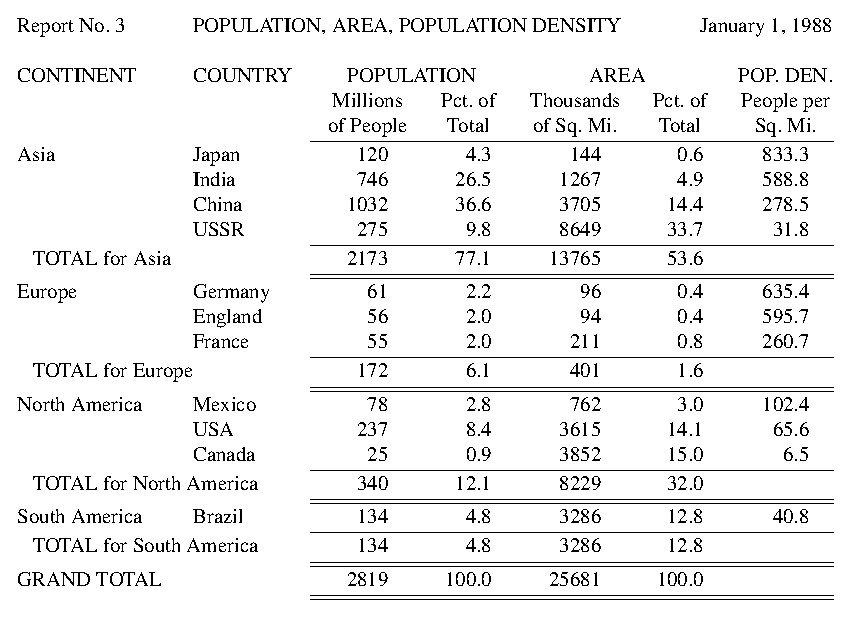
\includegraphics{./images/report3.eps}
\end{center}

如果可能的话, 我们建议构造一个程序来格式化表格, 实现一个像 \verb'tbl' 这样 
复杂的程序的确很有野心, 但不妨让我们从一个小程序开始: 这个程序以左对齐的
方式在列中打印文本条目, 其列宽度为所在列的最大值; 如果是数值则右对齐, 但是 
数值所占的域相对于本列最宽的项居中. 如果给定头部与输入文件
\filename{countries}, 程序的输出是\footnote{头部需要额外提供 --- 译者注}:
\begin{awkcode}
    COUNTRY   AREA   POPULATION   CONTINENT    
    USSR      8649       275      Asia         
    Canada    3852        25      North America
    China     3705      1032      Asia         
    USA       3615       237      North America
    Brazil    3286       134      South America
    India     1267       746      Asia         
    Mexico     762        78      North America
    France     211        55      Europe       
    Japan      144       120      Asia         
    Germany     96        61      Europe       
    England     94        56      Europe       
\end{awkcode}

程序的实现代码非常紧凑:
\marginpar{98}
\begin{awkcode}
    # table - simple table formatter

    BEGIN {
        FS = "\t"; blanks = sprintf("%100s", " ")
        number = "^[+-]?([0-9]+[.]?[0-9]*|[.][0-9]+)$"
    }

    {   row[NR] = $0
        for (i = 1; i <= NF; i++) {
            if ($i ~ number)
                nwid[i] = max(nwid[i], length($i))
            wid[i] = max(wid[i], length($i))
        }
    }

    END {
        for (r = 1; r <= NR; r++) {
            n = split(row[r], d)
            for (i = 1; i <= n; i++) {
                sep = (i < n) ? "   " : "\n"
                if (d[i] ~ number)
                    printf("%" wid[i] "s%s", numjust(i,d[i]), sep)
                else
                    printf("%-" wid[i] "s%s", d[i], sep)
            }
        }
    }

    function max(x, y) { return (x > y) ? x : y }

    function numjust(n, s) {   # position s in field n
        return s substr(blanks, 1, int((wid[n]-nwid[n])/2))
    }
\end{awkcode}
第一次遍历记录数据与每列的最大宽度, 第二次遍历 (位于 \END) 在适当的位置打印
每一项. 对字母项进行左对齐比较容易: 我们使用 \verb'wid[i]' (第 
\verb'i' 列的最大宽度) 为 \printf 构造格式字符串, 比如说, 如果列的最大宽度
是 10, 则第 \verb'i' 列的格式字符串就是 \verb'%-10s' (假设该列是字母项).

如果是数字项, 则要多做点工作: 第 \verb'i' 列的条目 \verb'v' 需要右对齐,
就像这样:
\begin{center}
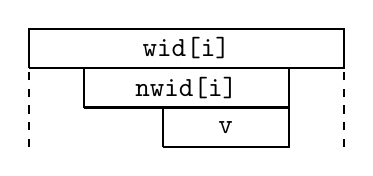
\begin{tikzpicture}
\draw[thick, dashed]
    (0.0, 0.0) -- (0.0, 1.0);
\draw[thick, dashed]
    (4.0, 0.0) -- (4.0, 1.0);

\draw[thick]
    (0.0, 1.0) -- (4.0, 1.0) -- (4.0, 1.5) -- (0.0, 1.5) -- (0.0, 1.0);

\draw[thick]
    (0.7, 0.5) -- (0.7, 1.0) -- (3.3, 1.0) -- (3.3, 0.5) -- (0.7, 0.5);

\draw[thick]
    (1.7, 0.0) -- (1.7, 0.5) -- (3.3, 0.5) -- (3.3, 0.0) -- (1.7, 0.0);

\node at (2.0, 1.25) {\texttt{wid[i]}};
\node at (2.0, 0.75) {\texttt{nwid[i]}};
\node at (2.5, 0.25) {\texttt{v}};
\end{tikzpicture}
\end{center}
\verb'v' 左边的空格数是 \verb'(wid[i]-nwid[i])/2', 所以 \verb'numjust' 会
在 \verb'v' 的末尾拼接这么多的空格, 然后再按照 \verb'%10s' 的格式输出 (假设 
该列的最大宽度是 10).

\marginpar{99}
\begin{exercise}
    \label{exer:form3_form4}
    修改 \verb'form3' 与 \verb'form4': 从别处获取日期, 而
    不是将日期硬编码到代码中.
\end{exercise}

\begin{exercise}
    由于四舍五入, 由 \verb'form3' 与 \verb'form4' 打印的项并不总是等于对应
    列的小计, 你会如何修正这个问题?
\end{exercise}

\begin{exercise}
    \label{exer:table_format}
    表格格式化程序假定所有数字的小数部分的位数都是相同的, 修改它, 使得即使 
    这个假定不成立, 程序也可以正确地工作.
\end{exercise}

\begin{exercise}
    增强 \verb'table' 的功能, 增强后的 \verb'table' 允许输入数据中出现一个
    格式说明行序列, 这个序列说明了如何格式化每一列随后的数据.
    (\texttt{tbl} 就是这样控制输出格式的)
\end{exercise}

\section{打包的查询与报表}
\label{sec:packaged_queries_and_reports}

如果某个查询经常被访问, 比较方便的做法是把它打包到一个命令中, 这样在下次
执行的时候, 就可以少打点字. 假设我们想要查询某个国家的人口, 面积, 以及人口 
密度, 比如说 Canada, 则可以键入 (假定用的是类Unix的 shell):
\begin{awkcode}
    awk '
    BEGIN { FS = "\t" }
    $1 ~ /Canada/ {
        printf("%s:\n", $1)
        printf("\t%d million people\n", $3)
        printf("\t%.3f million sq. mi.\n", $2/1000)
        printf("\t%.1f people per sq. mi.\n", 1000*$3/$2)
    }
    ' countries
\end{awkcode}
输出是 
\begin{awkcode}
    Canada:
        25 million people
        3.852 million sq. mi.
        6.5 people per sq. mi.
\end{awkcode}
现在, 如果我们想要查询其他国家的信息, 在执行每次查询前都需要修改国家的名称,
但是更方便的做法是把程序放入一个可执行文件中, 比如就叫 \verb'info',
查询时只要输入
\begin{awkcode}
    info Canada
    info USA
    ...
\end{awkcode}
我们可以利用 
\ref{sec:interaction_with_other_programs}
 节的技术, 把一个国家
的名称传递给程序, 或者, 我们也可以利用 shell, 把国家的名称放到适当的位置上:
\marginpar{100}
\begin{awkcode}
    awk '
    # info - print information about country
    #    usage: info country-name

    BEGIN { FS = "\t" }
    $1 ~ /'$1'/ {
        printf("%s:\n", $1)
        printf("\t%d million people\n", $3)
        printf("\t%.3f million sq. mi.\n", $2/1000)
        printf("\t%.1f people per sq. mi.\n", 1000*$3/$2)
    }
    ' countries
\end{awkcode}
程序开头的第二行
\begin{awkcode}
    $1 ~ /'$1'/
\end{awkcode}
第一个 \verb'$1' 指的是当前输入行的第一个字段, 而第二个 \verb'$1' (被单引号
包围着的)指的是国家名称参数, 也就是执行 shell 命令 \verb'info' 时的第一个参
数. 第二个 \verb'$1' 只对shell可见, 当命令被执行时, 它被 \verb'info' 后面 
的字符串所替代. 具体过程是: shell 通过拼接三个字符串来组合成 awk程序, 这三 
个字符串其中两个是被一对单引号包围起来的多行文本, 另外一个是 \verb'$1',
即 \texttt{info} 的参数. 需要注意的是, 可以把任意一个正则表达式传递给
\texttt{info}, 尤其是, 我们可以只给出国家名称的一部分, 或者一次指定多个国家
, 也可以查询到相关的国家信息, 比如 
\begin{awkcode}
    info 'Can|USA'
\end{awkcode}

\begin{exercise}
    \label{exer:info}
    修改 \texttt{info}: 参数通过 \texttt{ARGV} 传递进来, 而不是由 shell 
    进行替换.
\end{exercise}

\subsection{格式信函}
\label{subsec:form_letters}

Awk 也可以用于生成格式信函, 生成时
只需要用参数替换掉格式信函中的文本即可:
\begin{center}
\begin{tikzpicture}
\draw[thick, ->]
    (0.0, 0.5) -- (1.0, 0.5);
\draw[thick, ->]
    (3.0, 0.5) -- (4.0, 0.5);
\draw[thick, ->]
    (2.0, 2.0) -- (2.0, 1.0);

\draw[thick]
    (1.0, 0.0) -- (1.0, 1.0) -- (3.0, 1.0) -- (3.0, 0.0) -- (1.0, 0.0);

\node at (2.0, 2.3) {\texttt{letter.text}};
\node at (-0.7, 0.5) {参数值};
\node at (4.8, 0.5) {格式信函};
\node at (2.0, 0.5) {\texttt{form.gen}};
\end{tikzpicture}
\end{center}
格式信函的文本内容存放在文件 \filename{letter.text} 中,文本中包含了许多参
数, 只需要通过参数替换, 就可以生成不同内容的信函. 例如, 下面的文本使用了参数
\verb'#1' 到 \verb'#4', 这些参数分别表示国家名称, 人口, 面积, 以及人口密度:
\marginpar{101}
\begin{awkcode}
    Subject: Demographic Information About #1
    From: AWK Demographics, Inc.

    In response to your request for information about #1,
    our latest research has revealed that its population is #2
    million people and its area is #3 million square miles.
    This gives #1 a population density of #4 people per
    square mile.
\end{awkcode}

如果输入参数是
\begin{awkcode}
    Canada:25:3.852:6.5
\end{awkcode}
输出的的格式信函是:
\begin{awkcode}
    Subject: Demographic Information About Canada
    From: AWK Demographics, Inc.

    In response to your request for information about Canada,
    our latest research has revealed that its population is 25
    million people and its area is 3.852 million square miles.
    This gives Canada a population density of 6.5 people per
    square mile.
\end{awkcode}

程序 \verb'form.gen' 是格式信函生成程序:
\begin{awkcode}
    # form.gen - generate form letters
    #   input:  prototype file letter.text; data lines
    #   output: one form letter per data line

    BEGIN {
        FS = ":"
        while (getline <"letter.text" > 0) # read form letter
        form[++n] = $0
    }

    {   for (i = 1; i <= n; i++) { # read data lines
            temp = form[i]         # each line generates a letter
            for (j = NF; j >= 1; j--)
                gsub("#" j, $j, temp)
            print temp
        }
    }
\end{awkcode}

\verb'form.gen' 的 \BEGIN 从文件 \filename{letter.text} 中读取格式信函的
文本, 并存放到数组 \verb'form' 中, 剩下的工作是读取输入参数, 调用 
\verb'gsub' 将文本中的 \verb'#'\textit{n} 替换成对应的参数, 被修改的只 
是存储在数组 \verb'form' 中的信函副本, 文件 \filename{letter.text} 的内容
并没有发生改变. 注意程序是如何通过字符串拼接来生成 \verb'gsub' 的第一个
参数的.
\marginpar{102}

\section{关系数据库系统}
\label{sec:a_relational_database_system}

在这一节, 我们将会描述一个简单的关系型数据库系统, 这个系统的核心包括一个
类 awk 查询语言 \textit{q}, 一个数据字典 \filename{relfile}, 以
及一个查询处理程序 \verb'qawk', \verb'qawk' 的作用是把 \textit{q} 描述的
查询翻译成 awk 程序.

这个系统通过以下三种方式将 awk 扩展成一个数据库语言:
\begin{itemize}
    \item 字段通过名字来引用, 而不是数字.
    \item 数据库可以分散在多个文件中, 而不是限定在一个文件上.
    \item 可以交互性地生成一个查询序列.
\end{itemize}
使用名字 (而非数字) 引用字段的优势是显而易见的 --- \verb'$area' 看起来
比 \verb'$2' 更加自然, 但是, 把一个数据库分散存储在若干个文件中的优点
就没那么容易看出来. 多个文件组成的数据库维护起来更容易, 这主要是因为编辑
一个只含有少量字段的文件, 要比编辑一个包含全部字段的文件容易得多. 另外,
利用本节开发的数据库系统, 我们就有可能在不改变数据库访问程序的情况下,
重构数据库. 最后, 对于简单的查询来说, 访问一个小文件要比访问一个大文件高效
得多. 另一方面, 当我们往数据库添加数据时, 必须小心修改所有的相关文件, 
否则会带来一致性问题.

假设我们的数据库由一个单独
的文件 \filename{countries} 组成, 文件的每一行都包括四个字段, 字段的名字
分别是 \verb'country', \verb'area', \verb'population', 以及
\verb'continent'. 现在我们打算在数据库中新增一个文件 \filename{capitals},
文件的每一行都由两个字段组成 --- 国家及其首都:
\begin{awkcode}
    USSR    Moscow
    Canada  Ottawa
    China   Beijing
    USA     Washington
    Brazil  Brasilia
    India   New Delhi
    Mexico  Mexico City
    France  Paris
    Japan   Tokyo
    Germany Bonn
    England London
\end{awkcode}
与 \verb'countries' 一样, 字段之间用制表符分开.

从这两个文件出发, 如果我们想要打印位于亚洲的国家, 及其人口与首都, 那就必须
扫描这两个文件, 再拼凑出最终的结果. 举例来说, 如果输入数据不是很多, 下面
的程序就可以完成这件工作:
\marginpar{103}
\begin{awkcode}
    awk ' BEGIN { FS = "\t" }
          FILENAME == "capitals" {
              cap[$1] = $2
          }
          FILENAME == "countries" && $4 == "Asia" {
              print $1, $3, cap[$1]
          }
    ' capitals countries
\end{awkcode}

如果我们只需要输入
\begin{awkcode}
    $continent ~ /Asia/ { print $country, $population, $capital }
\end{awkcode}
就可以查询到亚洲国家的相关信息, 那将会非常的方便. 执行这条命令时, 有一个
程序会计算出字段的位置, 并将它们组成在一起, 这也是我们在 \textit{q} 中
短语化查询的方式, 接下来马上就会讨论到 \textit{q}.

\subsection{自然连接}
\label{subsec:natural_joins}

现在是时候讨论一些术语了. 在关系型数据库中, 一个文件被称为一张 \cterm{表} 
(\term{table}) 或一个 \cterm{关系} (\term{relation}), 把列叫作 \cterm{属性}
(\term{attribute}), 所以我们可以认为表格 \verb'capitals' 具有属性
\verb'country' 与 \verb'capital'.

一个 \cterm{自然连接} (\term{natural join}) (或简称为 \cterm{连接}) 指的是 
一个运算, 它将两张表以公共属性为基础组合成一张表, 这张表包含了两张表所有
的属性, 但是重复的属性会被移除. 如果我们把 \verb'countries' 与
\verb'capitals' 这两张表作自然连接, 我们就会得到一张新表 (姑且称为
\verb'cc'), 它的属性包括:
\begin{awkcode}
    country, area, population, continent, capital
\end{awkcode}
对于每一个同时出现在两张表中的国家来说, 我们都可以在 \verb'cc' 中找到一行
记录, 它包含了国家的名称, 后面跟着面积, 人口, 所在大洲,
以及国家的首都:
\begin{awkcode}
    Brazil  3286    134     South America	Brasilia
    Canada  3852    25      North America	Ottawa
    China   3705    1032    Asia                Beijing
    England 94      56      Europe              London
    France  211     55      Europe              Paris
    Germany 96      61      Europe              Bonn
    India   1267    746     Asia                New Delhi
    Japan   144     120     Asia                Tokyo
    Mexico  762     78      North America	Mexico City
    USA     3615    237     North America	Washington
    USSR    8649    275     Asia                Moscow
\end{awkcode}

我们实现连接运算的方法是根据它们的公共属性进行排序, 如果两张表的某一行的
公共属性值相同, 那就把它们合并起来, 就像上面这张表显示的那样. 为了处理
涉及到多张表的查询, 我们会先将表格作连接, 然后再对连接后的表作查询, 也就 
是说, 如果有必要的话, 我们会创建一个临时文件.
\marginpar{104}
为了响应查询:
\begin{awkcode}
    $continent ~ /Asia/ { print $country, $population, $capital }
\end{awkcode}
我们将 表 \verb'countries' 与 表 \verb'capitals'  作连接, 再将查询应用到
连接结果上, 通常来说, 完成这些操作最关键的地方在于将哪些表作连接.

实际的连接操作可以通过 Unix 命令 \texttt{join} 来完成, 但是如果系统上
没有该命令, 可以用这里提供的一个 用 awk 实现的简易版本. 它将两个文件按照
各自的第一个字段进行连接, 比如下面两张表

\begin{center}
\begin{tabular}{c|c|c}
    \hline
    \hline
    ATT1    & ATT2 & ATT3 \\
    \hline
    \texttt{A}       & \texttt{w}    & \texttt{p}    \\
    \texttt{B}       & \texttt{x}    & \texttt{q}   \\
    \texttt{B}      & \texttt{y}    & \texttt{r}    \\
    \texttt{C}      & \texttt{z}    & \texttt{s}    \\
    \hline
\end{tabular}
\hspace{2em}
\begin{tabular}{c|c}
    \hline
    \hline
    ATT1    & ATT4 \\
    \hline
    \texttt{A}       & \texttt{1}   \\  
    \texttt{A}       & \texttt{2}   \\
    \texttt{B}      & \texttt{3}    \\
    \hline
\end{tabular}
\end{center}

\vspace{1em}
作连接后得到
\vspace{1em}

\begin{center}
\begin{tabular}{c|c|c|c}
    \hline
    \hline
    ATT1        & ATT2  & ATT3   &   ATT4   \\
    \hline
    \texttt{A}  & \texttt{w}    & \texttt{p} &  \texttt{1}  \\
    \texttt{A}  & \texttt{w}    & \texttt{p} &  \texttt{2}  \\
    \texttt{B}  & \texttt{x}    & \texttt{q} &  \texttt{3}  \\
    \texttt{B}  & \texttt{y}    & \texttt{r} &  \texttt{3}  \\
\end{tabular}
\end{center}
\vspace{1em}

\texttt{join} 不假定输入表格是等长的, 但是它会认为表格是有序的, 互相匹配的
输入字段的每一种组合都会在输出中占据一行.
\begin{awkcode}
    # join - join file1 file2 on first field
    #   input:  two sorted files, tab-separated fields
    #   output: natural join of lines with common first field

    BEGIN {
        OFS = sep = "\t"
        file2 = ARGV[2]
        ARGV[2] = ""  # read file1 implicitly, file2 explicitly
        eofstat = 1   # end of file status for file2
        if ((ng = getgroup()) <= 0)
            exit      # file2 is empty
    }

    {   while (prefix($0) > prefix(gp[1]))
            if ((ng = getgroup()) <= 0)
                exit  # file2 exhausted
        if (prefix($0) == prefix(gp[1]))  # 1st attributes in file1
            for (i = 1; i <= ng; i++)     #     and file2 match
                print $0, suffix(gp[i])   # print joined line
    }

    function getgroup() { # put equal prefix group into gp[1..ng]
        if (getone(file2, gp, 1) <= 0)    # end of file
            return 0
        for (ng = 2; getone(file2, gp, ng) > 0; ng++)
            if (prefix(gp[ng]) != prefix(gp[1])) {
                unget(gp[ng])    # went too far
                return ng-1
            }
        return ng-1
    }

    function getone(f, gp, n) {  # get next line in gp[n]
        if (eofstat <= 0) # eof or error has occurred
            return 0
        if (ungot) {      # return lookahead line if it exists
            gp[n] = ungotline
            ungot = 0
            return 1
        }
        return eofstat = (getline gp[n] <f)
    }

    function unget(s)  { ungotline = s; ungot = 1 }
    function prefix(s) { return substr(s, 1, index(s, sep) - 1) }
    function suffix(s) { return substr(s, index(s, sep) + 1) }
\end{awkcode}
\marginpar{105}
执行 \verb'join' 时, 需要向它传递两个参数, 它们都表示输入文件名.
第一个属性值相同的行组成一个行组, 它们从第二个文件中读出, 如果第一个文件
的某一行的前缀与某些行组的公共属性值相同, 那么行组中的每一行都会出现在
输出中.

函数 \texttt{getgroup} 把下一组前缀相同的行放入数组 \texttt{gp} 中, 它调用
\texttt{getone} 来获取每一行, 如果发现获取到的行不属于本组, 就调用
\texttt{unget} 将它放回. 我们把提取第一个属性值的代码局限在函数
\texttt{prefix} 中, 这样以后改起来也比较方便.

读者应该注意一下函数 \texttt{getone} 与 \texttt{unget} 如何推回一个输入行.
在读取新行之前, \texttt{getone} 检查是否已经有一行被读取并由
\texttt{unget} 存放在某个变量中, 如果是, 则返回该行. 我们之前遇到过这类问
题: 在一次操作中, 读取了过多的输入. 推回是解决此类问题的另一种办法.
在本章早些时候出现的 control-break 程序中, 我们把处理操作延迟了, 而在这里,
通过一对函数, 我们假定不会看到额外的输入.

\begin{exercise}
    \label{exer:join}
    本节实现的 \texttt{join} 不会进行错误检查, 也不会检查文件是否是有序的.
    修复这些问题, 在修复之后, 程序会变得多大?
\end{exercise}

\begin{exercise}
    实现 \texttt{join} 的另一个版本, 它将一个文件整个读入内存, 然后再执行 
    连接操作. 与原来的版本相比, 哪个更简单?
\end{exercise}

\begin{exercise}
    修改 \texttt{join}: 它可以按照输入文件的任意一个字段或字段组来
    进行连接, 并可以按照任意的顺序, 有选择地输出某些字段.
\end{exercise}

\subsection{\texttt{relfile}}
\marginpar{106}
为了回答关于分散在多张表中的数据库的问题, 我们必须知道每张表中包含什么内容,
我们把这些信息存储在名为 \texttt{relfile} 的文件中 (``rel'' 指的是
``relation''). 文件 \texttt{relfile} 包含了数据库中每张表的名字, 属性,
如果表格不存在, 那么文件还包含了构造表格的规则. 文件 \texttt{relfile} 的
内容是一系列的表格描述符, 表格描述符具有形式:
\begin{pattern}
    \indent\textit{tablename} \par 
    \indent\indent\textit{attribute} \par 
    \indent\indent\textit{attribute} \par 
    \indent\indent\indent ...   \par
    \indent\indent\texttt{!}\textit{command} \par
    \indent\indent\indent ...
\end{pattern}
\textit{tablename} 与 \textit{attribute} 都是字符串, 在 \textit{tablename} 
之后是该表包含的属性名列表, 每一个属性名前面都有一个空格或制表符, 属性名
之后是可选 的命令序列, 命令以感叹号开始, 它说明了如何构造这张表格.
如果一张表不含构造命令, 则说明已经有一个文件以该表的名字命名, 且包含了
该表的数据, 这样的表叫做 \cterm{基表} (\term{base table}), 数据被插入
到基表中, 并在基表中更新. 在文件 \filename{relfile} 中, 如果某张表
在属性名之后出现了构造命令, 则称这张表是 \cterm{导出表} (\term{derived
table}), 只有在必要的时候才会构造导出表.

我们使用下面的 \filename{relfile} 来表示扩展了的国家数据库:
\begin{awkcode}
    countries:
        country
        area
        population
        continent
    capitals:
        country
        capital
    cc:
        country
        area
        population
        continent
        capital
        !sort countries >temp.countries
        !sort capitals >temp.capitals
        !join temp.countries temp.capitals >cc
\end{awkcode}
这个文件说明数据库中有两张基表 --- \filename{countries} 与
\filename{capitals}, 一张导出表 \filename{cc}, 导出表 \filename{cc} 通过 
把基表排序并存放在临时文件中, 再对临时文件执行连接操作来生成, 也就是说, 
\filename{cc} 通过执行
\marginpar{107}
\begin{awkcode}
    sort countries >temp.countries
    sort capitals >temp.capitals
    join temp.countries temp.capitals >cc
\end{awkcode}
生成.

一个 \texttt{relfile} 常常包含一张 \cterm{全局关系表} (\term{universal
relation}), 它是一张包含了所有属性的表, 是 \texttt{relfile} 的最后一张表,
这种做法保证至少有一张表包含了属性的所有可能的组合, 表格 \texttt{cc}
就是 数据库 countries-capitals 的全局关系表.

一个优秀的数据库设计必须考虑到该数据库可能收到的查询种类, 属性间存在的
依赖关系, 但是对于一个小数据库来说, \textit{q} 已经足够快了. 因为数据库
的表比较少, 所以很难展现出 \texttt{relfile} 设计的精妙之外.

\subsection{\textit{q}, 类 awk 查询语言}
\label{subsec:q_an_awk_like_query_language}

我们的数据库查询语言 \textit{q} 由单独一行的 awk 程序组成, 但字段名被属性名
替代. 查询处理程序 \texttt{qawk} 按照下面的步骤来响应一个查询:
\begin{enumerate}
	\item 判断该查询所包含的属性集;
	\item 从 \texttt{relfile} 的第一行开始, 搜索第一张包含了查询
	中全部属性
	的表, 如果该表是基表, 则用它作为查询的输入, 如果是导出表, 则构造
	该表, 再用它作为查询的输入. (这意味着查询中可能出现的属性组合
	一定也出现在 \texttt{relfile} 的基表或导出表中);
	\item 通过把符号型的字段引用替换成对应 的数值型字段引用, 将
	\textit{q} 查询转换成等价的 awk 程序, 这个程序接下来会把步骤 2 决定
	的表作为输入数据.
\end{enumerate}

\textit{q} 查询:
\begin{awkcode}
    $continent ~ /Asia/ { print $country, $population }
\end{awkcode}
提到了属性 \texttt{continent}, \texttt{country} 与 \texttt{population},
它们都是第一张表 \texttt{countries} 的属性子集. 查询处理程序把该查询转换
成程序 
\begin{awkcode}
    $4 ~ /Asia/ { print $1, $3 }
\end{awkcode}
并把文件 \filename{countries} 作为输入数据.

\textit{q} 查询 
\begin{awkcode}
    { print $country, $population, $capital }
\end{awkcode}
包含属性 \texttt{country}, \texttt{population} 与 \texttt{capital}, 它们 
都是导出表 \texttt{cc} 的属性子集. 于是查询处理程序利用 \filename{relfile}
列出的构造命令构造出表格 \texttt{cc}, 并将该查询转换成程序
\begin{awkcode}
    { print $1, $3, $5 }
\end{awkcode}
\marginpar{108}
程序把刚构造而成的 \texttt{cc} 作为输入数据.

虽然我们用的是 ``查询'' 这个词来描述 \texttt{qawk}, 但实际上它也可以用
来作计算, 下面这个查询打印面积的平均值:
\begin{awkcode}
    { area += $area }; END { print area/NR }
\end{awkcode}

\subsection{\texttt{qawk}, \textit{q}-to-awk 翻译器}
\label{subsec:qawk_a_q_to_awk_translator}

我们用 \texttt{qawk} 的实现来结束本章, 它把 \textit{q} 查询转换成等价的
awk 程序.

首先, \texttt{qawk} 读取文件 \filename{relfile}, 将表名收集到数组 
\texttt{relname} 中. 为了构造第 \textit{i} 张表, 程序把必要的构造命令
收集到数组 \texttt{array} 中, 从 \texttt{cmd[}\textit{i}\texttt{,}
\texttt{1]} 开始
存放. 它还把每张表的属性收集到2维数组 \texttt{attr} 中, 元素 \texttt{attr[}
\textit{i}\texttt{,}\texttt{a}\texttt{]} 存放的是第 \textit{i} 张表中,
名为 \textit{a} 的属性的索引.

然后, \texttt{qawk} 读取一个查询, 判断它会用到哪些属性, 查询中的属性都
是形式为 \verb'$'\textit{name} 的字符串. 利用函数 \texttt{subset}, 就可以 
找到第一张包含了查询中全部属性的表 $T_i$. 程序通过把属性的索引替换成
原始形式来生成 awk 程序, 并执行必要的命令来生成表格 $T_i$, 再执行 新生成
的awk程序, 把表格 $T_i$ 作为输入数据.

对每一个后来的查询, 第二个步骤都要重复一次, 下面这个流程图展示了 \texttt{qawk} 
的框架:
\begin{center}
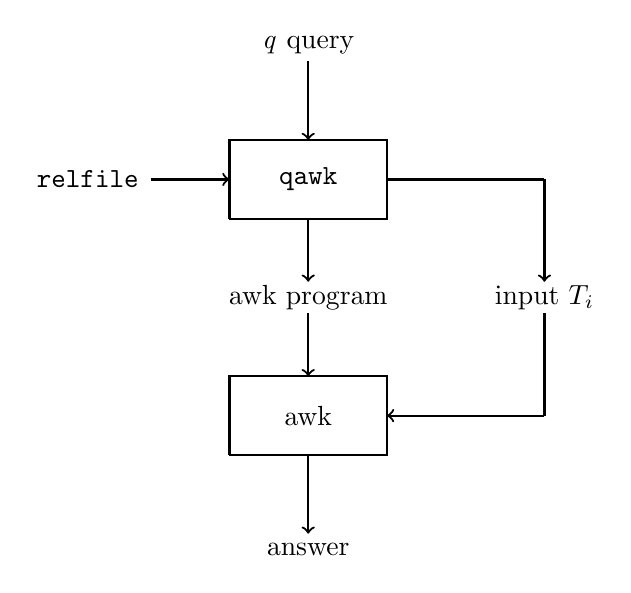
\begin{tikzpicture}
    \draw[thick] (0.0, 0.0) -- (2.0, 0.0) -- (2.0, 1.0) -- (0.0, 1.0)
    -- (0.0, 0.0);
    \draw[thick] (0.0, 3.0) -- (2.0, 3.0) -- (2.0, 4.0) -- (0.0, 4.0)
    -- (0.0, 3.0);

    \node at (1.0, 0.5) {awk};
    \node at (1.0, 3.5) {\texttt{qawk}};
    \node at (1.0, 2.0) {awk program};
    \node at (4.0, 2.0) {input $T_i$};
    \node at (1.0, -1.2) {answer};
    \node at (1.0, 5.2) {\textit{q} query};
    \node at (-1.8, 3.5) {\texttt{relfile}};

    \draw[thick,->] (-1.0, 3.5) -- (0.0, 3.5);
    \draw[thick,->] (1.0, 5.0) -- (1.0, 4.0);
    \draw[thick,->] (1.0, 3.0) -- (1.0, 2.2);
    \draw[thick,->] (1.0, 1.8) -- (1.0, 1.0);
    \draw[thick,->] (1.0, 0.0) -- (1.0, -1.0);
    \draw[thick] (2.0, 3.5) -- (4.0, 3.5);
    \draw[thick,->] (4.0, 3.5) -- (4.0, 2.2);
    \draw[thick] (4.0, 1.8) -- (4.0, 0.5);
    \draw[thick,->] (4.0, 0.5) -- (2.0, 0.5);
\end{tikzpicture}
\end{center}

\marginpar{109}
这是 \texttt{qawk} 的源代码:
\begin{awkcode}
    # qawk - awk relational database query processor

    BEGIN { readrel("relfile") }
    /./   { doquery($0) }

    function readrel(f) {
        while (getline <f > 0)   # parse relfile
            if ($0 ~ /^[A-Za-z]+ *:/) {     # name:
                gsub(/[^A-Za-z]+/, "", $0)  # remove all but name
                relname[++nrel] = $0
            } else if ($0 ~ /^[ \t]*!/)     # !command...
                cmd[nrel, ++ncmd[nrel]] = substr($0,index($0,"!")+1)
            else if ($0 ~ /^[ \t]*[A-Za-z]+[ \t]*$/)  # attribute
                attr[nrel, $1] = ++nattr[nrel]
            else if ($0 !~ /^[ \t]*$/)      # not white space
                print "bad line in relfile:", $0
    }
    function doquery(s,   i,j) {
        for (i in qattr)  # clean up for next query
            delete qattr[i]
        query = s    # put $names in query into qattr, without $
        while (match(s, /\$[A-Za-z]+/)) {
            qattr[substr(s, RSTART+1, RLENGTH-1)] = 1
            s = substr(s, RSTART+RLENGTH+1)
        }
        for (i = 1; i <= nrel && !subset(qattr, attr, i); ) 
            i++
        if (i > nrel)     # didn't find a table with all attributes
            missing(qattr)
        else {            # table i contains attributes in query
            for (j in qattr)   # create awk program
                gsub("\\$" j, "$" attr[i,j], query)
            for (j = 1; j <= ncmd[i]; j++)  # create table i
                if (system(cmd[i, j]) != 0) {
                    print "command failed, query skipped\n", cmd[i,j]
                    return
               }
            awkcmd = sprintf("awk -F'\t' '%s' %s", query, relname[i])
            printf("query: %s\n", awkcmd)   # for debugging
            system(awkcmd)
        }
    }
    function subset(q, a, r,   i) {  # is q a subset of a[r]?
        for (i in q)
            if (!((r,i) in a))
                return 0
        return 1
    }
    function missing(x,     i) {
        print "no table contains all of the following attributes:"
        for (i in x)
            print i
    }
\end{awkcode}

\marginpar{110}
\begin{exercise}
	如果你的系统不支持 awk 的 \texttt{system} 函数, 请修改
	\texttt{qawk}, 修改后的 \texttt{qawk} 把命令序列写入一个或多个文件
	中, 这些文件可以被单独地执行.
\end{exercise}

\begin{exercise}
    \label{exer:system}
	构造导出表的时候, \texttt{qawk} 为每一个命令调用一次
	\texttt{system}, 修改 \texttt{qawk}, 修改后的 \texttt{qawk} 把
	所有的构造表格的命令都收集到一个字符串中, 这样就可以只需要调用一次
	\texttt{system}. 
\end{exercise}

\begin{exercise}
    \label{exer:qawk}
	修改 \texttt{qawk}, 使得它可以检查即将作为输入数据的导出文件是否已经
	存在. 如果文件已经存在, 并且基文件在导出文件被导出之后未曾
	修改过, 那么我们就可以直接使用该导出文件, 而不用重新计算. 可以参考
	第 \ref{chap:experiments_with_algorithms} 章的程序 \texttt{make}.
\end{exercise}

\begin{exercise}
    \label{exer:multiline_query}
	提供一种输入并编辑多行查询的方式. 只要对 \texttt{qawk} 作些许修改,
	就可以把多行查询收集起来. 一种可选的方案是调用你喜欢的编辑器,
	另一种方式是用 awk 实现一个简单的编辑器.
\end{exercise}

\section{小结}
\label{sec:reports_and_databases_summary}
在这一章, 我们主要学习了如何使用 awk, 按照结构化的方式来访问和打印信息,
正好和 \ref{chap:data_processing} 章形成对照, 因为第
\ref{chap:data_processing} 章使用 awk 的方式都是专门针对某一具体的问题,
这种情况更加典型.

为了生成表格, ``分而治之'' 通常是最好的方法: 在一个程序中准备数据, 如果 
必要的话就对数据排序, 然后用第二个程序对数据进行格式化. Control break 可
以通过向前看, 或者推回输入 (通常是比较优雅的方式) 来处理. (有时候也可以
通过管道来完成这些工作, 虽然我们在这章没有用到.) 为了处理格式的细节, 相对
于手工计算字符个数, 一种更好的替代方案是用某些程序来完成机械化的部分.

虽然 awk 并不是数据库产品的工具, 但是对于小型的个人数据库来说, 它是一个
非常合理的选择, 而且在阐述某些数据库的基本概念方面, 它表现得也非常优秀,
为了论证这两点, 我们开发了 \texttt{qawk}.

\subsection*{参考资料}
关于数据库有着非常丰富的优秀书籍, 读者可以看一下 J. D. Ullman 的
\textit{Principles of Database Systems} (Computer Science Press, 1986).

